\section{Signature annotation scheme (Linux)}
\label{sign:linux}

%%%%%%%%%%%%%%%%%%%%%%%%%%%%%%%%%%%%%%%%%%%%%%%%%%%%%%%%%%%%%%%%%%%%%%%%%%%%%%%%
\subsection{Implementation}
\label{sign:linux:implementation}

\subsubsection{Network Integration}

Assuming that we can correctly construct a mapping between network traffic and endpoint process, we then need to manifest this correlation as a tag, annotated to each individual packet. For this tag, we decided to use a SHA256 Hash-based Message Authentication Code (HMAC-SHA256) with a pre-shared secret in order to provide endpoint authentication and if needed, payload integrity guarantees (limited to the payload due to the complexities of NAT traversal \cite{rfc6314}). We discarded digital signatures as an alternative early on due to having higher computational requirements and occupying more space than generally available for protocol options.

We note that in this version of \daf{}, the HMAC secrets are assumed to be shared between parties of an organization a priori. Any annotations sent to third parties that are not aware of our system should be silently filtered by the TCP/IP stack of the endhosts, as long as they \textit{correctly} implement the IP protocol. Key management, including secret sharing and revocation for compromised hosts are outside the scope of this paper and are the subject of future work.

In an effort to minimize overhead, we avoided solutions that would render the Internet Protocol no longer stateless (e.g., spanning the signature over multiple packets). However, doing so would have to be transparent to systems that are not compliant with our implementation. For example, appending the signature as part of the payload would indubitably break communication at the application layer. Although the 40-byte \textbf{IP Options} section is an adequate conduit for our 32-byte HMAC and can painlessly cover multiple Layer 4 protocols, we acquiesce that it raises concerns with regard to non-ICMP traffic traversal over the Internet \cite{fonseca2005ip, mantuchiroiuevaluationnetworkextensions, kazemian2012header, goodchild2017record}. In order to overcome this limitation, we examined the possibility of extending said annotation scheme to the transport layer:

\textbf{TCP Options:} Although almost universally accepted due to their impact on WAN performance (e.g., Selective Acknowledgement, Window Scaling, etc.) the limited 40-byte space \cite{john1981transmission} has made it essentially impossible to introduce new experimental options. If we followed the guideline to shared use of experimental option codepoints \cite{rfc6994}, our annotation would total 36 bytes, prohibiting the inclusion of other options. Although the TCP Extended Data Offset Option \cite{ietf-tcpm-tcp-edo-13} addresses this issue, it has been pending standardization since 2014. Existing studies \cite{trieu2015implementation} are also insufficient for assessing its viability.

\textbf{UDP Options:} In contrast to IP and TCP options, UDP options are a recent creation \cite{ietf-tsvwg-udp-options-23} that stemmed from a redundancy between the IP Total Length and UDP Length fields. While pending standardization since 2015, concerns have been raised regarding inconsistent behaviour observed in network equipment when calculating the L4 checksum \cite{zullo2020overcoming}. Although the Checksum Compensation Option \cite{fairhurst-udp-options-cco-00} has been proposed as a solution, there is still lacking evidence that this new protocol extension will be accepted in the wider Internet.

For these reasons, we considered it prudent to select \textbf{IP Options} over any Layer 4 alternative. We may revisit this decision once TCP EDO is standardized and UDP options receive sufficient testing over public networks.


\subsubsection{Packet interception and modification}

There are multiple methods of intercepting, filtering and modifying network traffic. Our implementation is based on the \texttt{NetfilterQueue} extension to the \texttt{Xtables} system. \texttt{NetfilterQueue} takes advantage of the \texttt{nfnetlink\_queue} kernel subsystem to deviate packets that match \texttt{iptables} rules through a userspace process. This delegates the selection of built-in targets (i.e., ACCEPT, DROP, etc.) that are to be applied, to said process. Once the userspace process subscribes to a certain queue and starts receiving packets, these can be analyzed in full (starting with the Layer 3 header), further deferred for judgement to a different process and optionally, be arbitrarily modified before their eventual reintroduction in kernel space.

This approach permits us to implement \texttt{iptables} extensions without requiring the user to load any additional kernel modules. Considering that this system was initially introduced in August 2005 as part of Linux 2.6.14, it is safe to assume that most current-day distributions support this feature. Loading kernel modules on the other hand, while providing better performance due to the reduced number of context switches (exacerbated in \texttt{NetfilterQueue} by the lack of zero-copy), may be difficult to achieve on some virtual cloud environments due to the kernel being in lockdown. Our decision to extend \texttt{iptables} and not other firewall alternatives is motivated primarily by its prominence in the industry. For example, LinkedIn recently implemented a distributed firewall \cite{linkedin_dfw} that manages host-bound filtering rules based on \texttt{iptables} and its predecessor, \texttt{ipset}. Aside from the performance disadvantage, the main flaw that applies to \texttt{iptables} in general, and translates to our solution as well, is the possibility to bypass the Netfilter kernel hooks by using the \texttt{PF\_PACKET} low-level socket interface. However, this operation necessitates root privileges on the part of the attacker. Consequently, this particular scenario falls outside the purview of our threat model.


\subsubsection{Integration with Xtables and snort3}

In order to leverage the benefits of \daf{} even on end hosts where it is not possible, or at least not practical to be deployed, we have implemented two out-of-tree extensions for \texttt{iptables} and \texttt{snort3}. The former consists of a shared object that implements the module-specific \texttt{iptables} frontend, and a \texttt{Xtables} kernel module that accomplishes the packet match evaluation. Because the latter operates in userspace and the packet retrieval is deferred to \texttt{libDAQ} (i.e., its data acquisition library), both functions are accomplished in the same resulting shared object (i.e., the IPS module). We note that neither extension requires its associated tool to be recompiled, both being dynamically loaded at runtime. In both cases, we consider a packet match to occur if the computed SHA256-HMAC over the Layer 4 payload (with a user-provided secret) corresponds to the contents of an experimental IP option found in the same packet.

%%%%%%%%%%%%%%%%%%%%%%%%%%%%%%%%%%%%%%%%%%%%%%%%%%%%%%%%%%%%%%%%%%%%%%%%%%%%%%%%
\subsection{Evaluation}
\label{sign:linux:evaluation}

The experimental setup and testing methodology applied to this traffic labling system is identical to that described in in Chapter \ref{appfw:daf}. The reason for this is that the system being evaluated was originally part of \daf{}.

\begin{figure}[h]
    \centering

    \begin{tikzpicture}
        \begin{axis}[
            width             = \textwidth,
            height            = 7cm,
            at                = {(0,0)},
            xmin              = 600,
            xmax              = 2000,
            ymin              = 300,
            xtick distance    = 200,
            grid              = both,
            xlabel            = {MTU [bytes]},
            ylabel            = {Throughput [Mbps]},
            legend style      = {at={(0.97,0.15)}, anchor=east},
            legend cell align = left,
        ]
            \addplot[color=Goldenrod, very thick]
                table[x=mtu, y=baseline, col sep=comma]
                {src/chapters/05-SignatureFirewall/data/nuc-throughput.csv};
            \addlegendentry{baseline}

            \addplot[color=NavyBlue, very thick]
                table[x=mtu, y=RUSu-pktsig, col sep=comma]
                {src/chapters/05-SignatureFirewall/data/nuc-epoll-multiple.csv};
            \addlegendentry{RUS+sig (epoll)}

            \addplot[color=OliveGreen, very thick]
                table[x=mtu, y=sigRUS-esorics, col sep=comma]
                {src/chapters/05-SignatureFirewall/data/nuc-throughput.csv};
            \addlegendentry{RUS+sig (io\_uring)}
        \end{axis}
    \end{tikzpicture}

    \caption{\daf{} throughput on Intel NUC with signature-based packet tagging.}
    \label{sign:linux:fig:nuc-throughput-new}
\end{figure}


In Figre \ref{sign:linux:fig:nuc-throughput} we observe the throughput of \daf{} on the Intel NUC mini-PC while using the \textit{Rescan prevention (R)}, \textit{Namespace Switch Skip (S)} and the \textit{Disabled cached object ordering (U)} performance optimizations. Additionally, each emitted packet is annotated with an experimental IP option containing a SHA-256 HMAC calculated over the Transport Layer payload. Because the \textit{Verdict Batching (B)} optimization would prevent the modification of the packet, it remains disabled in this battery of tests. We note that this is a limitation of the \texttt{NetfilterQueue} API and its use is incompatible with any form of packet annotation. In the aforementioned figure we illustrate the throughput of two different versions of \daf{}. While the original used the \texttt{epoll} notification system to multiplex input processing on multiple sockets, the current implementation utilizez the \texttt{io\_uring} system for achieving asynchronous I/O. The range of MTU values was limited to 2000 in order to better illustrate behavioural similarities between the two variants before reaching linerate, which is maintained for MTU values greater than 2000. The lower bound of 600 is motivated by relatively recent changes to the \texttt{e1000e} driver that enforce a minimum value of 604 bytes on a physical network interface.

\begin{figure}[h]
    \centering

    \begin{tikzpicture}
        \begin{axis}[
            width             = \textwidth,
            height            = 6cm,
            at                = {(0,0)},
            xmin              = 600,
            xmax              = 9300,
            ymin              = 0,
            xtick distance    = 2000,
            grid              = both,
            xlabel            = {MTU [bytes]},
            ylabel            = {Throughput [Mbps]},
            legend style      = {at={(0.97,0.15)}, anchor=east},
            legend cell align = left,
        ]
            \addplot[color=RoyalBlue, very thick]
                table[x=mtu, y=sigRUS-usenix, col sep=comma]
                {src/chapters/05-SignatureFirewall/data/cocos-throughput.csv};
            \addlegendentry{RUS+sig (epoll)}

            \addplot[color=OliveGreen, very thick]
                table[x=mtu, y=sigRUS-esorics, col sep=comma]
                {src/chapters/05-SignatureFirewall/data/cocos-throughput.csv};
            \addlegendentry{RUS+sig (io\_uring)}
        \end{axis}
    \end{tikzpicture}

    \caption{\daf{} throughput on the IBM system with signature-based packet tagging.}
    \label{sign:linux:fig:cocos-throughput}
\end{figure}


While no definitive conclusion could be drawn from the Intel NUC experiments as to the superiority of the \texttt{io\_uring} variant over the \texttt{epoll}-based one, Figure \ref{sign:linux:fig:cocos-throughput} can provide sufficient proof in support of this claim. For the IBM system, we observe that the asynchronous implementation outperforms the \texttt{epoll}-based one from the outset. Since the overall throughput stabilizes at approx. 800 Mbps, we decided against plotting the baseline for comparison. Because this baseline would be roughly one degree of magnitude larger, certain features would become obfuscated. For example, we notice periodic and gradual gains in throughput at lower MTUs at intervals of approx. 256 bytes. Although these were present in the Intel NUC experiments as well, the data captured on the IBM system is less noisy. At higher MTU values however, we observe indicators of aliasing, where increases in packet size result in immediate throughput upsurges followed by gradual decreases, in periodic patterns. Additionally, we observe momentary downgrades in throughput within 40-byte ranges of MTU starting at 1550, 3600 and 7690. Noting that the MTU step in our experiments is of 10 bytes, we surmise that these anomalies occur within 2048 and 4096 byte increases from one another, respectively. Since these are present in both the Intel NUC and IBM system experiments, we can deduce that they are unrelated to the network interface controller hardware or driver. Furthermore, there are present in our packet annotation benchmarks but not in our previous firewalling tests. As a result, they are also not caused by particularities of the Linux TCP/IP stack, but instead by the \texttt{NetfilterQueue} packet overwrite mechanism. Specifically, the addition of the experimental IP option that consists of 32 bytes leads to an overflow of the default send buffer which in turn results in a packet buffer resize and possible reallocation.

%%%%%%%%%%%%%%%%%%%%%%%%%%%%%%%%%%%%%%%%%%%%%%%%%%%%%%%%%%%%%%%%%%%%%%%%%%%%%%%%
\subsection{Discussion}
\label{sign:linux:discussion}

\subsubsection{Key management using GNU Privacy Guard}
\label{sign:linux:discussion:gpg}

GNU Privacy Guard (GPG) is one of the more prevalent implementations of the OpenPGP standard \cite{rfc4880}, adhering to the "web of trust" model, rather than the Public Key Infrastructure (PKI) \cite{maurer1996modelling} alternative. Early in the development of our prototype, we considered employing \texttt{GPGME} for the more sensitive cryptographic operations. \texttt{GPGME} is a wrapper library over the OpenPGP backend, and constitutes the recommended method of integrating GPG functionalities into other applications. The primary reason why we chose GPG stands in its key and identity management mechanisms. The identity of the user is inextricably linked to his or her private key. At that time, we intended to allow the user to lend our firewall access to this private key by means of the GPG agent (a keystore caching daemon). In doing so, we would avoid retaining the private key in the memory of a yet-untested prototype.

Nonetheless, we quickly realized that \texttt{GPGME} could not be a permanent solution. While some library calls only change internal states (e.g.: selecting the pinentry mode or cryptographic engine), active key selection as well as signature generation and verification spawn multiple background processes which \texttt{exec()} on each individual query. Although the intended cryptographic operations are in and of themselves computationally taxing, repeatedly spawning new processes for each packet would ultimately prove impractical.


\subsubsection{Netfilter Queue bug}
\label{sign:linux:discussion:bug}

During the development of our \texttt{iptables} module for \daf{}'s integration in existing environments, we discovered an inssue with how the NetfilterQueue kernel module handles changes to its packet buffer.

Whenever a packet matches a Netfilter rule with a NFQ target, it is temporarily placed in the receive buffer of a netlink socket. Even when a process reads this packet into userspace (partially or integrally) for the purpose of performing Deep Packet Inspection, a copy of the packet will still reside in kernel space pending a verdict. If affirmative, the stored packet is reinjected into the kernel network stack with a minimal amount of memory copy operations. However, when the verdict is predicated on overwriting the packet buffer with a version specified by the deciding process, certain fields of the \texttt{sk\_buff} structure can be rendered invalid.

Whenever we inject an IP options section on verdict transmission, we effectively increase the size of the Layer 3 header by a maximum of 40 bytes. Consequently, the Layer 4 header is shifted relative to the beginning of the Network header. Normally this would not pose a problem, especially after the packet is emitted from the local system. Nonetheless, during the development of our \texttt{iptables} plugin, we discovered that using the \texttt{tcp\_hdr()} macro to obtain a reference to the TCP header would yield incorrect results on the originating system but not on other endpoints. We initially wanted to test the soundness of our implementation by matching the packet that we modified on the OUTPUT chain on its way out, on the POSTROUTING chain with a LOG jump target.

\begin{figure}
    \centering
    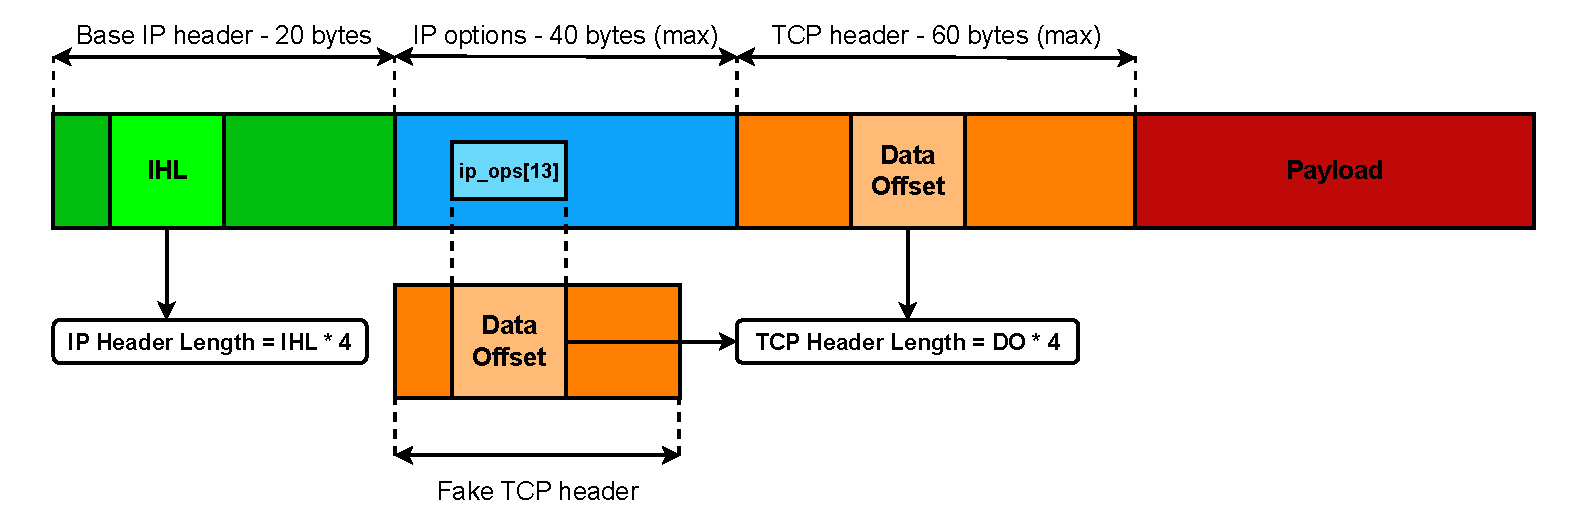
\includegraphics[width=\textwidth,keepaspectratio]{figures/daf-nfq-bug.pdf}
    \caption{TCP header mismatch due to IP header resize with NFQ.}
    \label{appfw:daf:fig:nfq-bug}
\end{figure}

However, the recommended API for accessing the Transport header would calculate its location based on the value of the \texttt{transport\_header} field that is stored in the \texttt{sk\_buff} structure. Since the \texttt{NetfilterQueue} kernel module does not account for variable protocol header sizes, this field remains unchanged. The result is that our Layer 4 payload digest was being calculated on a buffer whose starting position was incorrect (see Fig. \ref{appfw:daf:fig:nfq-bug}). Instead of adding the Data Offset (as number of dwords) to the start of the TCP header (which is dependent on the true length of the IP header), a random number that coincided with a high nibble in the stored SHA256 HMAC (the $33^{rd}$ byte in the updated IP header) was instead used as offset from the \textit{base} IP header. This lead to a mismatch during the HMAC verification.

Not only could this have resulted in an illegal memory access albeit in very specific circumstances, but other Xtables modules that make reference to Layer 4 fields may potentially be susceptible to this issue. Although it would be hard for a malicious user to mount an attack using this bug, we surmise that one could inject a fake TCP header as a 20-byte IP options section. Any POSTROUTING rules (e.g. network address translation) would end up matching the fake fields instead of the actual header. At the moment it is unclear how this vulnerability could be further leveraged to benefit a potential attacker or whether it needs to be patched. Because it does not directly relate to the issue at hand, we decided to revisit it at a later time.

